\providecommand{\main}{../..}
\documentclass[\main/thesis.tex]{subfiles}
\begin{document}

\section{The Next Numeral}\label{next}

Paul Benacerraf once argued\cite{benacerraf1965numbers} that, there are two kinds
of \textit{counting} which correspond to \textbf{transitive} and \textbf{intransitive}
uses of the verb ``to count.'' Transitive counting, in his sense, is to assign one
of the numbers to the cardinality of a set, by establishing a one-to-one correspondence
between the numbers and the objects one is counting, all the way from none to
all. Intransitive counting, on the other hand, is to generate a sequence of
notation, that could go as far as we need. And it seems that one can only learn
how to count intransitively first, before knowning how to count transitively,
but not vice versa. So it is important to know how to generate the next numeral
we need.

\subsection{What does it mean by ``The Next''?}

When mapping some systems such as {\lstinline|Numeral 10 5 0|} onto
the natural numbers, their number lines appear to be ``gapped'' because their
evaluations are not \textit{surjective}.
The number ``6'', for example, has no correspondence on the numeral side.

\begin{center}
    \begin{adjustbox}{max width=\textwidth}
        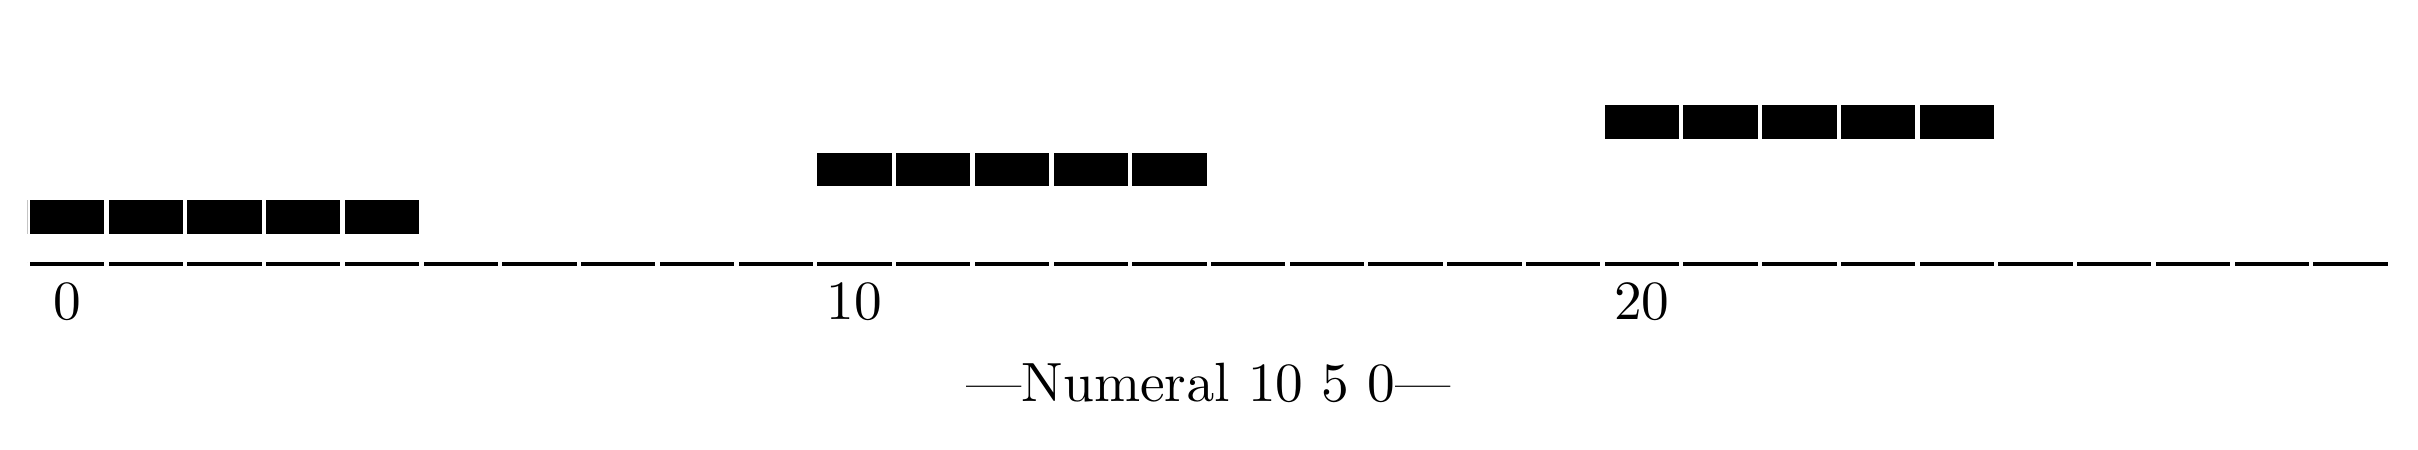
\begin{tikzpicture}
            % the frame
            \path[clip] (0, -2) rectangle (30, 3);
            % the spine
            \draw[ultra thick] (0,0) -- (30,0);

            % % the body
            \foreach \i in {0,...,2} {
                \draw[thick, fill=black] ({\i * 10}, {\i * 0.6 + 0.4}) rectangle ({\i * 10 + 5}, {\i * 0.6 + 0.8});
            };

            % ticks
            \foreach \i in {0,...,30} {
                \draw[ultra thick, draw=white] (\i,-0.3) -- (\i,3);
            };
            %
            % labels
            \node[below, scale=2] at (0.5, 0) {$0$};
            \node[below, scale=2] at (10.5, 0) {$10$};
            \node[below, scale=2] at (20.5, 0) {$20$};
            \node[scale=2] at (15, -1.5) {{\lstinline|Numeral 10 5 0|}};
        \end{tikzpicture}
    \end{adjustbox}
\end{center}

Whilst systems such as {\lstinline|Numeral 10 15 0|} map more than one numeral
onto the same number. We can see immediately that their evaluations are not
\textit{injective} as those number lines ``overlap'' with each other.

\begin{center}
    \begin{adjustbox}{max width=\textwidth}
        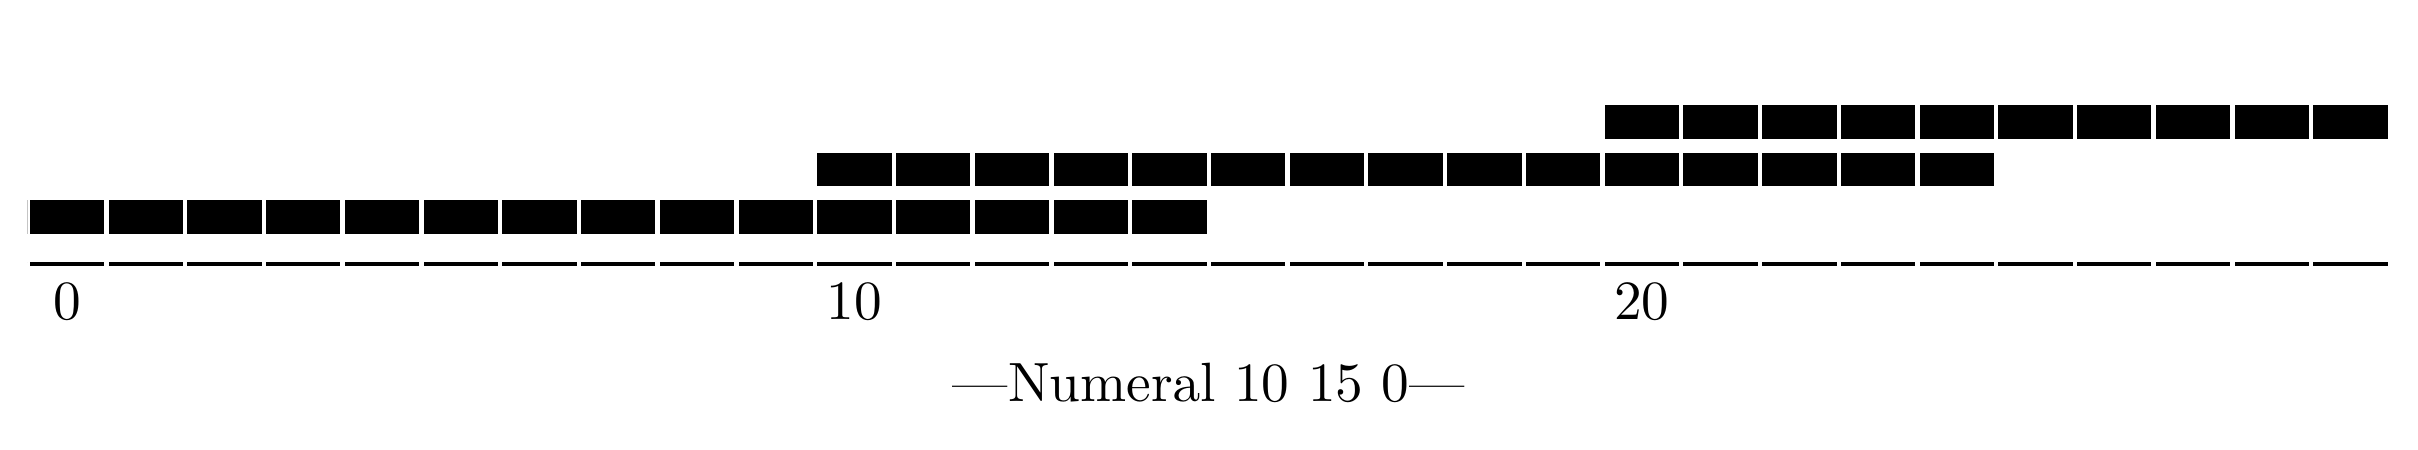
\begin{tikzpicture}
            % the frame
            \path[clip] (0, -2) rectangle (30, 3);
            % the spine
            \draw[ultra thick] (0,0) -- (30,0);

            % % the body
            \foreach \i in {0,...,2} {
                \draw[thick, fill=black] ({\i * 10}, {\i * 0.6 + 0.4}) rectangle ({\i * 10 + 15}, {\i * 0.6 + 0.8});
            };

            % ticks
            \foreach \i in {0,...,30} {
                \draw[ultra thick, draw=white] (\i,-0.3) -- (\i,3);
            };
            %
            % labels
            \node[below, scale=2] at (0.5, 0) {$0$};
            \node[below, scale=2] at (10.5, 0) {$10$};
            \node[below, scale=2] at (20.5, 0) {$20$};
            \node[scale=2] at (15, -1.5) {{\lstinline|Numeral 10 15 0|}};
        \end{tikzpicture}
    \end{adjustbox}
\end{center}


As we can see, numerals do not align with numbers perfectly.
Finding ``the next number'' thus becomes a non-trivial problem.
Therefore, we define the next numeral as \textbf{the least numeral that is greater than itself}.

\subsection{Implementation}

Given a numeral, say {\lstinline|xs|}, to find the next numeral of {\lstinline|xs|},
it reasonable to expect that {\lstinline|xs|} must not be a maximum.
Otherwise, there would exist no such a numeral that is \textit{greater than itself}.

Again, the indices are classified by {\lstinline|numView|} into four categories.
The case of {\lstinline|NoDigits|} and {\lstinline|AllZeros|} are rather trivial.
We focus on the other two.

\begin{lstlisting}
next-numeral : ∀ {b d o}
    → (xs : Numeral b d o)
    → ¬ (Maximum xs)
    → Numeral b d o
next-numeral {b} {d} {o} xs ¬max with numView b d o
next-numeral xs ¬max | NullBase d o = ?
next-numeral xs ¬max | NoDigits b o = NoDigits-explode xs
next-numeral xs ¬max | AllZeros b   =
    contradiction (Maximum-AllZeros xs) ¬max
next-numeral xs ¬max | Proper b d o proper = ?
\end{lstlisting}

\subsection{Validating the Implementation}

To validate the correctness of the implementation of {\lstinline|next-numeral|},
i.e., to make sure that the function does return a numeral that is:

\begin{enumerate}
    \item greater than the given numeral
    \item the least of all such numerals
\end{enumerate}

We need to prove these two propositions:

\begin{lstlisting}
next-numeral-is-greater : ∀ {b d o}
    → (xs : Numeral b d o)
    → (¬max : ¬ (Maximum xs))
    → ⟦ next-numeral xs ¬max ⟧ > ⟦ xs ⟧
\end{lstlisting}

\begin{lstlisting}
next-numeral-is-immediate : ∀ {b d o}
    → (xs : Numeral b d o)
    → (ys : Numeral b d o)
    → (¬max : ¬ (Maximum xs))
    → ⟦ ys ⟧ > ⟦ xs ⟧
    → ⟦ ys ⟧ ≥ ⟦ next-numeral xs ¬max ⟧
\end{lstlisting}

We come up with the name ``immediate''
because ``the least numeral that is greater than itself'' is a bit too wordy.

\subsection{Outline}

We are going to finish programs and proofs of systems of {\lstinline|NullBase|}
and {\lstinline|Proper|} respectively.

\begin{itemize}
    \item {\lstinline|NullBase|}
        \begin{enumerate}
            \item {\lstinline|next-numeral-NullBase|}
            \item {\lstinline|next-numeral-is-greater-NullBase|}
            \item {\lstinline|next-numeral-is-immediate-NullBase|}
        \end{enumerate}
    \item {\lstinline|Proper|}
        \begin{itemize}
            \item {\lstinline|next-numeral-Proper|}
            \item {\lstinline|next-numeral-is-greater-Proper|}
            \item {\lstinline|next-numeral-is-immediate-Proper|}
        \end{itemize}
\end{itemize}

However, programs and proofs of systems of {\lstinline|Proper|} will be defined
\textit{simultaneously} with mutually recursive definitions.
The reason why we need the property {\lstinline|next-numeral-is-greater-Proper|}
in the first place is that they are neccessary for implementing
{\lstinline|next-numeral-Proper|}.

\subsection{The Next Numeral of NullBase}

To find the next numeral of systems of {\lstinline|NullBase|},
all we have to do is to manipulate the LSD.
Since only the value of the LSD has effect on the evaluation.
All numerals are mapped onto this single and continuous number line below.

\begin{center}
    \begin{adjustbox}{max width=\textwidth}
        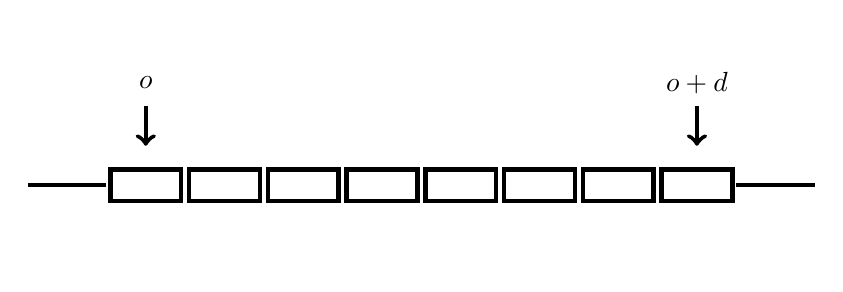
\begin{tikzpicture}
            % the frame
            \path[clip] (0, -1) rectangle (10, 2);
            % the spine
            \draw[ultra thick] (0,0) -- (1,0);
            \draw[ultra thick] (9,0) -- (10,0);
            % the body

            \foreach \i in {1,...,8} {
                \draw[ultra thick, fill=white] ({\i+0.05}, -0.2) rectangle ({\i+0.95}, +0.2);
            };

            % labels
            \draw[->, ultra thick] (1.5,1) -- (1.5,0.5)
                node at (1.5, 1.3) {$o$};
            \draw[->, ultra thick] (8.5,1) -- (8.5,0.5)
                node at (8.5, 1.3) {$o+d$};
        \end{tikzpicture}
    \end{adjustbox}
\end{center}

Finding the next numeral is as simple as incrementing the LSD.
To make room for the increment, numerals that are mapped onto the rightmost
number of the line have to be excluded.

\begin{center}
    \begin{adjustbox}{max width=\textwidth}
        \begin{tikzpicture}
            % the frame
            \path[clip] (0, -1) rectangle (10, 2);
            % the spine
            \draw[ultra thick] (0,0) -- (1,0);
            \draw[ultra thick] (9,0) -- (10,0);
            % the body

            \foreach \i in {1,...,7} {
                \draw[ultra thick, fill=black] ({\i+0.05}, -0.2) rectangle ({\i+0.95}, +0.2);
            };
            \draw[ultra thick, fill=gray] (8.05, -0.2) rectangle (8.95, +0.2);

            % labels
            \draw[->, ultra thick] (1.5,1) -- (1.5,0.5)
                node at (1.5, 1.3) {$o$};
            \draw[->, ultra thick] (7.5,1) -- (7.5,0.5)
                node at (7.5, 1.3) {$o+d-1$};

            % arrows
            \foreach \i in {0,...,9} {
                \coordinate (\i) at ({\i + 0.5}, -0.3);
            };
            \foreach \i in {1,...,7} {
                \pgfmathsetmacro{\j}{\i + 1}
                \path[->, ultra thick] (\i) edge[bend right=60] node {} ($ (\j) + (-0.1, 0) $);
            };
        \end{tikzpicture}
    \end{adjustbox}
\end{center}

\subsubsection{{\lstinline|next-numeral-NullBase|}}

Numerals with the greatest LSD are first ruled out because they also happen
to be maxima. The rest of the numerals are then pattern matched to have their
LSDs replaced with an incremented one.

\begin{lstlisting}
next-numeral-NullBase : ∀ {d o}
    → (xs : Numeral 0 (suc d) o)
    → ¬ (Maximum xs)
    → Numeral 0 (suc d) o
next-numeral-NullBase xs       ¬max with Greatest? (lsd xs)
next-numeral-NullBase xs       ¬max | yes greatest
    = contradiction (Maximum-NullBase-Greatest xs greatest) ¬max
next-numeral-NullBase (x ∙)    ¬max | no ¬greatest
    = digit+1 x ¬greatest ∙
next-numeral-NullBase (x ∷ xs) ¬max | no ¬greatest
    = digit+1 x ¬greatest ∷ xs
\end{lstlisting}

\subsubsection{Lemma}

Instead of proving that {\lstinline|next-numeral-NullBase|} does compute a numeral
that is:
\begin{enumerate}
    \item greater than the given numeral
    \item the least of all such numerals
\end{enumerate}

We prove a stronger proposition, that {\lstinline|next-numeral-NullBase|} would
compute the \textit{successor} of the given number.

\begin{lstlisting}[basicstyle=\ttfamily\scriptsize]
next-numeral-NullBase-lemma : ∀ {d o}
    → (xs : Numeral 0 (suc d) o)
    → (¬max : ¬ (Maximum xs))
    → ⟦ next-numeral-NullBase xs ¬max ⟧ ≡ suc ⟦ xs ⟧
next-numeral-NullBase-lemma {d} {o} xs    ¬max with Greatest? (lsd xs)
next-numeral-NullBase-lemma {d} {o} xs    ¬max | yes greatest =
    contradiction (Maximum-NullBase-Greatest xs greatest) ¬max
next-numeral-NullBase-lemma {d} {o} (x ∙) ¬max | no ¬greatest =
    begin
        ⟦ digit+1 x ¬greatest ∙ ⟧
    ≡⟨ refl ⟩
        Digit-toℕ (digit+1 x ¬greatest) o
    ≡⟨ digit+1-toℕ x ¬greatest ⟩
        suc (Fin.toℕ x + o)
    ≡⟨ refl ⟩
        suc ⟦ x ∙ ⟧
    ∎
next-numeral-NullBase-lemma {d} {o} (x ∷ xs) ¬max | no ¬greatest =
    begin
        ⟦ digit+1 x ¬greatest ∷ xs ⟧
    ≡⟨ refl ⟩
        Digit-toℕ (digit+1 x ¬greatest) o + ⟦ xs ⟧ * zero
    ≡⟨ cong (λ w → w + ⟦ xs ⟧ * zero) (digit+1-toℕ x ¬greatest) ⟩
        suc (Fin.toℕ x + o + ⟦ xs ⟧ * zero)
    ≡⟨ refl ⟩
        suc ⟦ x ∷ xs ⟧
    ∎
\end{lstlisting}

\subsubsection{{\lstinline|next-numeral-is-greater-NullBase|}}

Recall that {\lstinline|x < y|} is essentially a synonym of {\lstinline|suc x ≤ y|}.
We nail this with the lemma we have just proven.

\begin{lstlisting}
next-numeral-is-greater-NullBase : ∀ {d o}
    → (xs : Numeral 0 (suc d) o)
    → (¬max : ¬ (Maximum xs))
    → ⟦ next-numeral-NullBase xs ¬max ⟧ > ⟦ xs ⟧
next-numeral-is-greater-NullBase xs ¬max =
    start
        suc ⟦ xs ⟧
    ≈⟨ sym (next-numeral-NullBase-lemma xs ¬max) ⟩
        ⟦ next-numeral-NullBase xs ¬max ⟧
    □
\end{lstlisting}

\subsubsection{{\lstinline|next-numeral-is-immediate-NullBase|}}

Here, the argument {\lstinline|ys|} stands for \textit{any} numeral of {\lstinline|Numeral 0 (suc d) o|}.

\begin{lstlisting}
next-numeral-is-immediate-NullBase : ∀ {d o}
    → (xs : Numeral 0 (suc d) o)
    → (ys : Numeral 0 (suc d) o)
    → (¬max : ¬ (Maximum xs))
    → ⟦ ys ⟧ > ⟦ xs ⟧
    → ⟦ ys ⟧ ≥ ⟦ next-numeral-NullBase xs ¬max ⟧
next-numeral-is-immediate-NullBase xs ys ¬max prop =
    start
        ⟦ next-numeral-NullBase xs ¬max ⟧
    ≈⟨ next-numeral-NullBase-lemma xs ¬max ⟩
        suc ⟦ xs ⟧
    ≤⟨ prop ⟩
        ⟦ ys ⟧
    □
\end{lstlisting}

\subsection{The Next Numeral of Proper}

Unlike in systems of {\lstinline|NullBase|} where every numeral gets mapped onto
a single and continuous number line.
There are \textit{three different cases} where the given numeral might be located
in systems of {\lstinline|Proper|}.

\paragraph{Intervals}

This is the simplest case like in {\lstinline|NullBase|}.
The given numeral's LSD is not located at the end of the number line.

\begin{center}
    \begin{adjustbox}{max width=\textwidth}
        \begin{tikzpicture}
            % the frame
            \path[clip] (5.5, -1.5) rectangle (17.5, 1.5);

            % the body
            \foreach \i in {0,...,2} {
                \foreach \j in {0,...,5} {
                    \draw[ultra thick, fill=black] ({\i*8+\j+0.05}, {\i*0.6-0.8}) rectangle ({\i*8+\j+0.95}, {\i*0.6-0.4});
                };
                \draw[ultra thick, fill=gray] ({\i*8+6.05}, {\i*0.6-0.8}) rectangle ({\i*8+6.95}, {\i*0.6-0.4});
            };

            \foreach \i in {5,...,6} {
                \coordinate (\i) at ({\i + 0.5}, -0.9);
            };
            \foreach \i in {8,...,15} {
                \coordinate (\i) at ({\i + 0.5}, -0.3);
            };
            \foreach \i in {16,...,17} {
                \coordinate (\i) at ({\i + 0.5}, 0.3);
            };

            \foreach \i in {5,...,5} {
                \pgfmathsetmacro{\j}{\i + 1}
                \path[->, ultra thick] (\i) edge[bend right=60] node {} ($ (\j) + (-0.1, 0) $);
            };
            \foreach \i in {8,...,13} {
                \pgfmathsetmacro{\j}{\i + 1}
                \path[->, ultra thick] (\i) edge[bend right=60] node {} ($ (\j) + (-0.1, 0) $);
            };
            \foreach \i in {16,...,16} {
                \pgfmathsetmacro{\j}{\i + 1}
                \path[->, ultra thick] (\i) edge[bend right=60] node {} ($ (\j) + (-0.1, 0) $);
            };

        \end{tikzpicture}
    \end{adjustbox}
\end{center}

\paragraph{Gapped Endpoints}

When the given numeral's LSD happens to be the greatest
and there is a \textit{gap} before the next numeral.
There are no other numerals in between that could bridge the gap.

\begin{center}
    \begin{adjustbox}{max width=\textwidth}
        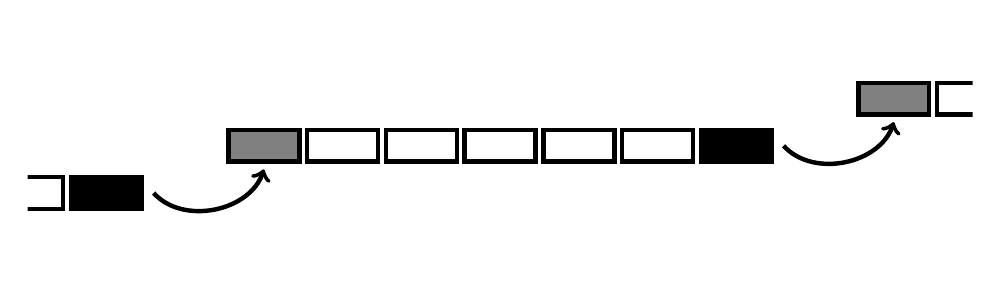
\begin{tikzpicture}
            % the frame
            \path[clip] (5.5, -1.5) rectangle (17.5, 1.5);

            % the body
            \foreach \i in {0,...,2} {
                \draw[ultra thick, fill=gray] ({\i*8+0.05}, {\i*0.6-0.8}) rectangle ({\i*8+0.95}, {\i*0.6-0.4});
                \foreach \j in {1,...,5} {
                    \draw[ultra thick] ({\i*8+\j+0.05}, {\i*0.6-0.8}) rectangle ({\i*8+\j+0.95}, {\i*0.6-0.4});
                };
                \draw[ultra thick, fill=black] ({\i*8+6.05}, {\i*0.6-0.8}) rectangle ({\i*8+6.95}, {\i*0.6-0.4});
            };

            % arrows
            \coordinate (A) at (7.1, -0.6);
            \coordinate (B) at (8.5, -0.3);
            \coordinate (C) at (15.1, 0);
            \coordinate (D) at (16.5, 0.3);

            \path[->, ultra thick] (A) edge[bend right=60] node {} (B);
            \path[->, ultra thick] (C) edge[bend right=60] node {} (D);
            % \path[->, ultra thick] (\i) edge[bend right=60] node {} ($ (\j) + (-0.1, 0) $);

        \end{tikzpicture}
    \end{adjustbox}
\end{center}

\paragraph{Ungapped Endpoints}

When the given numeral's LSD happens to be the greatest
but we can find another numeral right ahead of it.

% Just like in the case of \textit{gapped endpoints}, the rest of the numeral are
% replace with its next numeral.

% To reach the next numeral, the LSD has to be reset to the least digit;
% the rest of the numeral (digits of higher significance) are replaced with
% its \texit{next} numeral to compensate for the loss of the LSD.

\begin{center}
    \begin{adjustbox}{max width=\textwidth}
        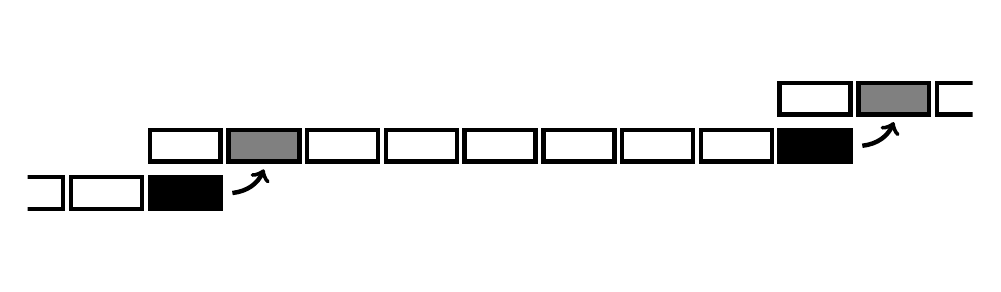
\begin{tikzpicture}
            % the frame
            \path[clip] (6.5, -1.5) rectangle (18.5, 1.5);

            % the body
            \foreach \i in {0,...,2} {
                \draw[ultra thick] ({\i*8+0.05}, {\i*0.6-0.8}) rectangle ({\i*8+0.95}, {\i*0.6-0.4});
                \draw[ultra thick, fill=gray] ({\i*8+1.05}, {\i*0.6-0.8}) rectangle ({\i*8+1.95}, {\i*0.6-0.4});
                \foreach \j in {2,...,7} {
                    \draw[ultra thick] ({\i*8+\j+0.05}, {\i*0.6-0.8}) rectangle ({\i*8+\j+0.95}, {\i*0.6-0.4});
                };
                \draw[ultra thick, fill=black] ({\i*8+8.05}, {\i*0.6-0.8}) rectangle ({\i*8+8.95}, {\i*0.6-0.4});
            };

            % arrows
            \coordinate (A) at (9.1, -0.6);
            \coordinate (B) at (9.5, -0.3);
            \coordinate (C) at (17.1, 0);
            \coordinate (D) at (17.5, 0.3);

            \path[->, ultra thick] (A) edge[bend right] node {} (B);
            \path[->, ultra thick] (C) edge[bend right] node {} (D);
            % \path[->, ultra thick] (\i) edge[bend right=60] node {} ($ (\j) + (-0.1, 0) $);

        \end{tikzpicture}
    \end{adjustbox}
\end{center}

\subsubsection{Gaps}

It is easy to tell if a given numeral is located in intervals or at endpoints
just by looking at its LSD.
However, to tell apart from \textit{gapped} and \textit{ungapped} endpoints
is an entirely different story.
First things first, we need a proposition for expressing this matter.

Given a numeral {\lstinline|x ∷ xs|} of {\lstinline|Numeral b d o|} and
suppose that the next numeral of {\lstinline|xs|} is {\lstinline|xs'|}.
The value of {\lstinline|x ∷ xs|} ranges from {\lstinline|⟦ xs ⟧ × b + o|} to
{\lstinline|⟦ xs ⟧ × b + o + d - 1|}.

\begin{center}
    \begin{adjustbox}{max width=\textwidth}
        \begin{tikzpicture}
            % the frame
            \path[clip] (4.5, -1.5) rectangle (18.5, 2.5);

            % ticks and labels
            \draw[ultra thick, dotted] (8.5,-1) -- (8.5,1)
                node[above] {{\lstinline|⟦ xs ⟧ × b + o|}};

            \draw[ultra thick, dotted] (16.5,-1) -- (16.5,1)
                node[above] {{\lstinline|⟦ xs' ⟧ × b + o|}};

            \draw[ultra thick, decoration={brace,mirror,raise=10},decorate]
                (8,-0.2) -- node[below=0.5] {totally {\lstinline|d|} digits} (14,-0.2);

            % the body
            \foreach \i in {0,...,2} {
                \foreach \j in {0,...,5} {
                    \draw[ultra thick, draw=gray, fill=white] ({\i*8+\j+0.05}, {\i*0.6-0.8}) rectangle ({\i*8+\j+0.95}, {\i*0.6-0.4});
                };
            };

        \end{tikzpicture}
    \end{adjustbox}
\end{center}

If we look closely, we can see that the gap comes from the difference between
{\lstinline|⟦ xs ⟧ × b + o + d|} and {\lstinline|⟦ xs' ⟧ × b + o|}.

\begin{center}
    \begin{adjustbox}{max width=\textwidth}
        \begin{tikzpicture}
            % the frame
            \path[clip] (37.5, -3.5) rectangle (55.5, 4.5);


            % ticks
            \draw[ultra thick, loosely dotted] (43.5,-1.5) -- (43.5,3)
                node[above, scale=1.5] {{\lstinline|⟦ xs ⟧ × b + o + d|}};

            \draw[ultra thick, loosely dotted] (49.5,-1.5) -- (49.5,3)
                node[above, scale=1.5] {{\lstinline|⟦ xs' ⟧ × b + o|}};

            \draw[ultra thick, decoration={brace,mirror,raise=10},decorate]
                (43.5,-1.5) -- node[below=0.5, scale=1.5] {{\lstinline|the gap|}} (49.5,-1.5);

            % the body
            \foreach \i in {0,...,2} {
                \foreach \j in {0,...,5} {
                    \draw[ultra thick, draw=gray, fill=white] ({\i*24+\j*3+0.15}, {\i*1.8-2.4}) rectangle ({\i*24+\j*3+2.85}, {\i*1.8-1.2});
                };
            };
        \end{tikzpicture}
    \end{adjustbox}
\end{center}

If there are enough digits to bridge the gap between {\lstinline|⟦ xs ⟧ × b + o|}
and {\lstinline|⟦ xs' ⟧ × b + o|} then there will be no gaps.
Thus the predicate for determine if there is a gap ahead of {\lstinline|x ∷ xs|}
can then be expressed as below. Notice that {\lstinline|next-numeral-Proper|}
is used as part of the definition.

\begin{lstlisting}
Gapped : ∀ b d o
    → (xs : Numeral (suc b) (suc d) o)
    → (proper : 2 ≤ suc (d + o))
    → Set
Gapped b d o xs proper
    = suc d < (⟦ next-numeral-Proper xs proper ⟧ ∸ ⟦ xs ⟧) * suc b
\end{lstlisting}

However, the predicate above does not take numerals like {\lstinline|x ∙|} into
account, i.e., numerals that are composed of only a single digit.
In that case, the gap ahead will be \textit{the first gap} among the others.
The predicate of the first gap is as simple as comparing the number of digits
{\lstinline|d|} with {\lstinline|carry o × b|}, where {\lstinline|carry o = 1 ⊔ o|}
computes the least (be greater than zero) digit of higher significance.

\begin{lstlisting}
Gapped : ∀ b d o → Set
Gapped b d o = suc d < carry o * suc b
\end{lstlisting}

Combining the two predicates above together, we devise a predicate for
predicting the gap ahead of a numeral.

\begin{lstlisting}
Gapped#0 : ∀ b d o → Set
Gapped#0 b d o = suc d < carry o * suc b

Gapped#N : ∀ b d o
    → (xs : Numeral (suc b) (suc d) o)
    → (proper : 2 ≤ suc (d + o))
    → Set
Gapped#N b d o xs proper
    = suc d < (⟦ next-numeral-Proper xs proper ⟧ ∸ ⟦ xs ⟧) * suc b

Gapped : ∀ {b d o}
    → (xs : Numeral (suc b) (suc d) o)
    → (proper : 2 ≤ suc (d + o))
    → Set
Gapped {b} {d} {o} (x ∙)    proper = Gapped#0 b d o
Gapped {b} {d} {o} (x ∷ xs) proper = Gapped#N b d o xs proper
\end{lstlisting}

Along with decidable versions.

\begin{lstlisting}
Gapped#0? :  ∀ b d o → Dec (Gapped#0 b d o)
Gapped#N? :  ∀ b d o
    → (xs : Numeral (suc b) (suc d) o)
    → (proper : 2 ≤ suc (d + o))
    → Dec (Gapped#N b d o xs proper)
Gapped? : ∀ {b d o}
    → (xs : Numeral (suc b) (suc d) o)
    → (proper : 2 ≤ suc (d + o))
    → Dec (Gapped {b} {d} {o} xs proper)
\end{lstlisting}

There is an important theorem about the intriguing relation between
{\lstinline|Gapped#0|} and {\lstinline|Gapped#N|} which will be proven and used
in later chapters.

\subsubsection{A View within another}

With the predicate {\lstinline|Gapped|} and its friends, we can further classify
systems of {\lstinline|Proper|} into finer categories.

\begin{lstlisting}[basicstyle=\ttfamily\scriptsize]
data NextView : (b d o : ℕ) (xs : Numeral b d o) (proper : 2 ≤ d + o) → Set where
    Interval : ∀ b d o
        → {xs : Numeral (suc b) (suc d) o}
        → {proper : 2 ≤ suc (d + o)}
        → (¬greatest : ¬ (Greatest (lsd xs)))
        → NextView (suc b) (suc d) o xs proper
    GappedEndpoint : ∀ b d o
        → {xs : Numeral (suc b) (suc d) o}
        → {proper : 2 ≤ suc (d + o)}
        → (greatest : Greatest (lsd xs))
        → (gapped : Gapped xs proper)
        → NextView (suc b) (suc d) o xs proper
    UngappedEndpoint : ∀ b d o
        → {xs : Numeral (suc b) (suc d) o}
        → {proper : 2 ≤ suc (d + o)}
        → (greatest : Greatest (lsd xs))
        → (¬gapped : ¬ (Gapped xs proper))
        → NextView (suc b) (suc d) o xs proper
\end{lstlisting}

\begin{lstlisting}[basicstyle=\ttfamily\scriptsize]
nextView : ∀ {b d o}
    → (xs : Numeral (suc b) (suc d) o)
    → (proper : 2 ≤ suc (d + o))
    → NextView (suc b) (suc d) o xs proper
nextView {b} {d} {o} xs proper with Greatest? (lsd xs)
nextView {b} {d} {o} xs proper | yes greatest with Gapped? xs proper
nextView {b} {d} {o} xs proper | yes greatest | yes gapped
    = GappedEndpoint  b d o greatest gapped
nextView {b} {d} {o} xs proper | yes greatest | no ¬gapped
    = UngappedEndpoint b d o greatest ¬gapped
nextView {b} {d} {o} xs proper | no ¬greatest
    = Interval b d o ¬greatest
\end{lstlisting}

\subsubsection{{\lstinline|next-numeral-Proper|}}

Finally, to compute the next numeral of systems of {\lstinline|Proper|},
we categorize the given numeral with {\lstinline|NextView|}
and delegate the task to corresponding helper functions.

\begin{lstlisting}[basicstyle=\ttfamily\scriptsize]
next-numeral-Proper : ∀ {b d o}
    → (xs : Numeral (suc b) (suc d) o)
    → (proper : 2 ≤ suc (d + o))
    → Numeral (suc b) (suc d) o
next-numeral-Proper xs proper with nextView xs proper
next-numeral-Proper xs proper | Interval b d o ¬greatest
    = next-numeral-Proper-Interval xs ¬greatest proper
next-numeral-Proper xs proper | GappedEndpoint b d o greatest gapped
    = next-numeral-Proper-GappedEndpoint xs proper gapped
next-numeral-Proper xs proper | UngappedEndpoint b d o greatest ¬gapped
    = next-numeral-Proper-UngappedEndpoint xs greatest proper ¬gapped
\end{lstlisting}

\paragraph{Interval}

\begin{center}
    \begin{adjustbox}{max width=\textwidth}
        \begin{tikzpicture}
            % the frame
            \path[clip] (5.5, -1.5) rectangle (17.5, 1.5);

            % the body
            \foreach \i in {0,...,2} {
                \foreach \j in {0,...,5} {
                    \draw[ultra thick, fill=black] ({\i*8+\j+0.05}, {\i*0.6-0.8}) rectangle ({\i*8+\j+0.95}, {\i*0.6-0.4});
                };
                \draw[ultra thick, fill=gray] ({\i*8+6.05}, {\i*0.6-0.8}) rectangle ({\i*8+6.95}, {\i*0.6-0.4});
            };

            \foreach \i in {5,...,6} {
                \coordinate (\i) at ({\i + 0.5}, -0.9);
            };
            \foreach \i in {8,...,15} {
                \coordinate (\i) at ({\i + 0.5}, -0.3);
            };
            \foreach \i in {16,...,17} {
                \coordinate (\i) at ({\i + 0.5}, 0.3);
            };

            \foreach \i in {5,...,5} {
                \pgfmathsetmacro{\j}{\i + 1}
                \path[->, ultra thick] (\i) edge[bend right=60] node {} ($ (\j) + (-0.1, 0) $);
            };
            \foreach \i in {8,...,13} {
                \pgfmathsetmacro{\j}{\i + 1}
                \path[->, ultra thick] (\i) edge[bend right=60] node {} ($ (\j) + (-0.1, 0) $);
            };
            \foreach \i in {16,...,16} {
                \pgfmathsetmacro{\j}{\i + 1}
                \path[->, ultra thick] (\i) edge[bend right=60] node {} ($ (\j) + (-0.1, 0) $);
            };

        \end{tikzpicture}
    \end{adjustbox}
\end{center}

To reach the next numeral, all we have to do is to increment the LSD.
There is no need of performing carries or messing with other digits.

\begin{lstlisting}[basicstyle=\ttfamily\scriptsize]
next-numeral-Proper-Interval : ∀ {b d o}
    → (xs : Numeral (suc b) (suc d) o)
    → (¬greatest : ¬ (Greatest (lsd xs)))
    → (proper : 2 ≤ suc (d + o))
    → Numeral (suc b) (suc d) o
next-numeral-Proper-Interval (x ∙)    ¬greatest proper
    = digit+1 x ¬greatest ∙
next-numeral-Proper-Interval (x ∷ xs) ¬greatest proper
    = digit+1 x ¬greatest ∷ xs
\end{lstlisting}

\paragraph{Gapped Endpoints}

\begin{center}
    \begin{adjustbox}{max width=\textwidth}
        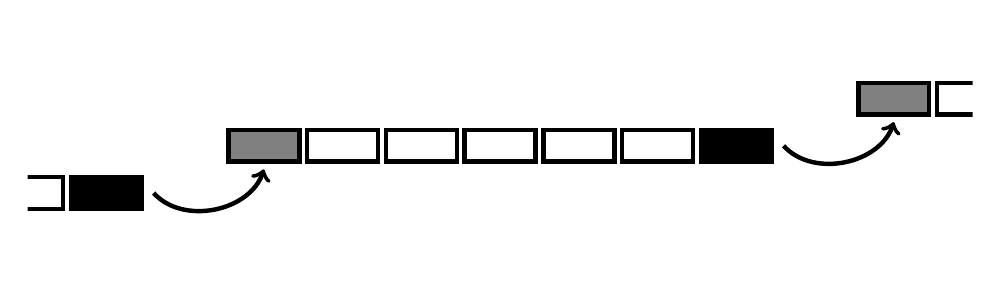
\begin{tikzpicture}
            % the frame
            \path[clip] (5.5, -1.5) rectangle (17.5, 1.5);

            % the body
            \foreach \i in {0,...,2} {
                \draw[ultra thick, fill=gray] ({\i*8+0.05}, {\i*0.6-0.8}) rectangle ({\i*8+0.95}, {\i*0.6-0.4});
                \foreach \j in {1,...,5} {
                    \draw[ultra thick] ({\i*8+\j+0.05}, {\i*0.6-0.8}) rectangle ({\i*8+\j+0.95}, {\i*0.6-0.4});
                };
                \draw[ultra thick, fill=black] ({\i*8+6.05}, {\i*0.6-0.8}) rectangle ({\i*8+6.95}, {\i*0.6-0.4});
            };

            % arrows
            \coordinate (A) at (7.1, -0.6);
            \coordinate (B) at (8.5, -0.3);
            \coordinate (C) at (15.1, 0);
            \coordinate (D) at (16.5, 0.3);

            \path[->, ultra thick] (A) edge[bend right=60] node {} (B);
            \path[->, ultra thick] (C) edge[bend right=60] node {} (D);
            % \path[->, ultra thick] (\i) edge[bend right=60] node {} ($ (\j) + (-0.1, 0) $);

        \end{tikzpicture}
    \end{adjustbox}
\end{center}

To reach the next numeral, the LSD is reset to the least digit;
the rest of the numeral (digits of higher significance) are replaced accordingly
compensate for the loss of the LSD.

\begin{lstlisting}[basicstyle=\ttfamily\scriptsize]
next-numeral-Proper-GappedEndpoint : ∀ {b d o}
    → (xs : Numeral (suc b) (suc d) o)
    → (proper : 2 ≤ suc (d + o))
    → (gapped : Gapped xs proper)
    → Numeral (suc b) (suc d) o
next-numeral-Proper-GappedEndpoint (x ∙)    proper gapped
    = z ∷ carry-digit d o proper ∙
next-numeral-Proper-GappedEndpoint (x ∷ xs) proper gapped
    = z ∷ next-numeral-Proper xs proper
\end{lstlisting}

\paragraph{Ungapped Endpoints}

\begin{center}
    \begin{adjustbox}{max width=\textwidth}
        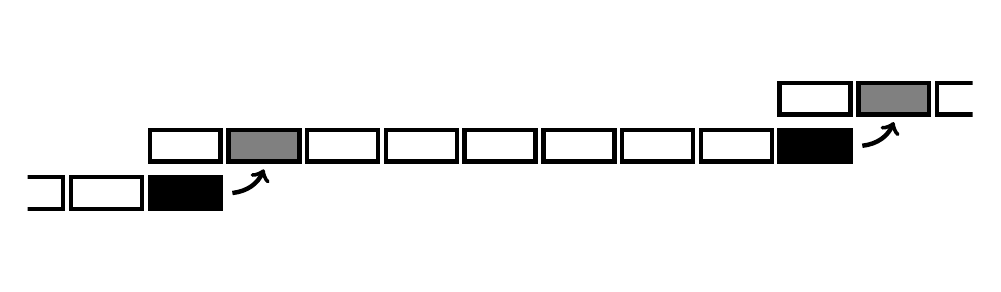
\begin{tikzpicture}
            % the frame
            \path[clip] (6.5, -1.5) rectangle (18.5, 1.5);

            % the body
            \foreach \i in {0,...,2} {
                \draw[ultra thick] ({\i*8+0.05}, {\i*0.6-0.8}) rectangle ({\i*8+0.95}, {\i*0.6-0.4});
                \draw[ultra thick, fill=gray] ({\i*8+1.05}, {\i*0.6-0.8}) rectangle ({\i*8+1.95}, {\i*0.6-0.4});
                \foreach \j in {2,...,7} {
                    \draw[ultra thick] ({\i*8+\j+0.05}, {\i*0.6-0.8}) rectangle ({\i*8+\j+0.95}, {\i*0.6-0.4});
                };
                \draw[ultra thick, fill=black] ({\i*8+8.05}, {\i*0.6-0.8}) rectangle ({\i*8+8.95}, {\i*0.6-0.4});
            };

            % arrows
            \coordinate (A) at (9.1, -0.6);
            \coordinate (B) at (9.5, -0.3);
            \coordinate (C) at (17.1, 0);
            \coordinate (D) at (17.5, 0.3);

            \path[->, ultra thick] (A) edge[bend right] node {} (B);
            \path[->, ultra thick] (C) edge[bend right] node {} (D);
            % \path[->, ultra thick] (\i) edge[bend right=60] node {} ($ (\j) + (-0.1, 0) $);

        \end{tikzpicture}
    \end{adjustbox}
\end{center}

Just like in the case of \textit{gapped endpoints}, the more significant part
of the numeral is replaced with something greater (either a carry-digit or
the next numeral).
The LSD is incremented and then subtracted by \textit{the exact size of the coming gap}.
To compute the size of the gap, it is necessary to compute {\lstinline|next-xs|},
the next numeral of the more significant part, beforehand.
Moreover, we also need to assure that {\lstinline|next-xs|} is greater than
{\lstinline|xs|}.
Hence these constructions have to be written as mutually recursive definitions.

\begin{lstlisting}[basicstyle=\ttfamily\scriptsize]
next-numeral-Proper-UngappedEndpoint : ∀ {b d o}
    → (xs : Numeral (suc b) (suc d) o)
    → (greatest : Greatest (lsd xs))
    → (proper : 2 ≤ suc (d + o))
    → (¬gapped : ¬ (Gapped xs proper))
    → Numeral (suc b) (suc d) o
next-numeral-Proper-UngappedEndpoint {b} {d} {o} (x ∙) greatest proper gapped
    = digit+1-n x greatest gap lower-bound ∷ carry-digit d o proper ∙
    where
        gap : ℕ
        gap = carry o * suc b

        lower-bound : gap > 0
        lower-bound = ...
next-numeral-Proper-UngappedEndpoint {b} {d} {o} (x ∷ xs) greatest proper gapped
    = digit+1-n x greatest gap lower-bound ∷ next-xs
    where
        gap : ℕ
        gap = (⟦ next-numeral-Proper xs proper ⟧ ∸ ⟦ xs ⟧) * suc b

        lower-bound : gap > 0
        lower-bound =  ... next-numeral-is-greater-Proper xs proper ...
\end{lstlisting}

\subsubsection{Lemmata}

These lemmata desctibe the relations between a given numeral and its next of
each category.

\paragraph{Remark} Here we show only the propositions because their proofs contain
some whopping ~200 lines of equational and preorder reasoning.

\begin{lstlisting}[basicstyle=\ttfamily\scriptsize]
next-numeral-Proper-Interval-lemma : ∀ {b d o}
    → (xs : Numeral (suc b) (suc d) o)
    → (¬greatest : ¬ (Greatest (lsd xs)))
    → (proper : 2 ≤ suc (d + o))
    → ⟦ next-numeral-Proper-Interval xs ¬greatest proper ⟧ ≡ suc ⟦ xs ⟧
\end{lstlisting}

\begin{lstlisting}[basicstyle=\ttfamily\scriptsize]
next-numeral-Proper-GappedEndpoint-lemma : ∀ {b d o}
    → (xs : Numeral (suc b) (suc d) o)
    → (greatest : Greatest (lsd xs))
    → (proper : 2 ≤ suc (d + o))
    → (gapped : Gapped xs proper)
    → ⟦ next-numeral-Proper-GappedEndpoint xs proper gapped ⟧ > suc ⟦ xs ⟧
\end{lstlisting}

\begin{lstlisting}[basicstyle=\ttfamily\scriptsize]
next-numeral-Proper-UngappedEndpoint-lemma : ∀ {b d o}
    → (xs : Numeral (suc b) (suc d) o)
    → (greatest : Greatest (lsd xs))
    → (proper : 2 ≤ suc (d + o))
    → (¬gapped : ¬ (Gapped xs proper))
    → ⟦ next-numeral-Proper-UngappedEndpoint xs greatest proper ¬gapped ⟧
        ≡ suc ⟦ xs ⟧
\end{lstlisting}

\subsubsection{{\lstinline|next-numeral-is-greater-Proper|}}

With lemmata above, proving {\lstinline|next-numeral-is-greater-Proper|} becomes
an easy task.

\begin{lstlisting}[basicstyle=\ttfamily\scriptsize]
next-numeral-is-greater-Proper : ∀ {b d o}
    → (xs : Numeral (suc b) (suc d) o)
    → (proper : 2 ≤ suc (d + o))
    → ⟦ next-numeral-Proper xs proper ⟧ > ⟦ xs ⟧
next-numeral-is-greater-Proper xs proper with nextView xs proper
next-numeral-is-greater-Proper xs proper | Interval b d o ¬greatest =
    start
        suc ⟦ xs ⟧
    ≈⟨ sym (next-numeral-Proper-Interval-lemma xs ¬greatest proper) ⟩
        ⟦ next-numeral-Proper-Interval xs ¬greatest proper ⟧
    □
next-numeral-is-greater-Proper xs proper | GappedEndpoint b d o greatest gapped =
    start
        suc ⟦ xs ⟧
    ≤⟨ n≤1+n (suc ⟦ xs ⟧) ⟩
        suc (suc ⟦ xs ⟧)
    ≤⟨ next-numeral-Proper-GappedEndpoint-lemma xs greatest proper gapped ⟩
        ⟦ next-numeral-Proper-GappedEndpoint xs proper gapped ⟧
    □
next-numeral-is-greater-Proper xs proper | UngappedEndpoint b d o greatest ¬gapped =
    start
        suc ⟦ xs ⟧
    ≈⟨ sym (next-numeral-Proper-UngappedEndpoint-lemma xs greatest proper ¬gapped) ⟩
        ⟦ next-numeral-Proper-UngappedEndpoint xs greatest proper ¬gapped ⟧
    □
\end{lstlisting}

\subsubsection{{\lstinline|next-numeral-is-immediate-Proper|}}

This proof also follows the same pattern, except that the case of
{\lstinline|GappedEndpoint|} becomes more complicated as its corresponding lemma
establishes only a preorder relation.

\begin{lstlisting}[basicstyle=\ttfamily\scriptsize]
next-numeral-is-immediate-Proper : ∀ {b d o}
    → (xs : Numeral (suc b) (suc d) o)
    → (ys : Numeral (suc b) (suc d) o)
    → (proper : 2 ≤ suc (d + o))
    → ⟦ ys ⟧ > ⟦ xs ⟧
    → ⟦ ys ⟧ ≥ ⟦ next-numeral-Proper xs proper ⟧
next-numeral-is-immediate-Proper xs ys proper prop with nextView xs proper
next-numeral-is-immediate-Proper xs ys proper prop | Interval b d o ¬greatest =
    start
        ⟦ next-numeral-Proper-Interval xs ¬greatest proper ⟧
    ≈⟨ next-numeral-Proper-Interval-lemma xs ¬greatest proper ⟩
        suc ⟦ xs ⟧
    ≤⟨ prop ⟩
        ⟦ ys ⟧
    □
next-numeral-is-immediate-Proper xs (y ∙) proper prop
    | GappedEndpoint b d o greatest gapped
    = contradiction prop $ >⇒≰ $
        start
            suc ⟦ y ∙ ⟧
        ≤⟨ s≤s (greatest-of-all o (lsd xs) y greatest) ⟩
            suc (Digit-toℕ (lsd xs) o)
        ≤⟨ s≤s (lsd-toℕ xs) ⟩
            suc ⟦ xs ⟧
        □
next-numeral-is-immediate-Proper (x ∙) (y ∷ ys) proper prop
    | GappedEndpoint b d o greatest gapped =
    start
        ⟦ z ∷ carry-digit d o proper ∙ ⟧
    ≤⟨ ... ⟩
        o + carry o * suc b
    ≤⟨ n+-mono o (*n-mono (suc b) ys-lower-bound) ⟩
        o + ⟦ ys ⟧ * suc b
    ≤⟨ ... ⟩
        ⟦ y ∷ ys ⟧
    □
    where
        ys-lower-bound : ⟦ ys ⟧ ≥ carry o
        ys-lower-bound = ...
next-numeral-is-immediate-Proper (x ∷ xs) (y ∷ ys) proper prop
    | GappedEndpoint b d o greatest gapped =
    start
        ⟦ z ∷ next-numeral-Proper xs proper ⟧
    ≤⟨ ... ⟩
        o + ⟦ next-numeral-Proper xs proper ⟧ * suc b
    ≤⟨ n+-mono o (*n-mono (suc b) ⟦next-xs⟧≤⟦ys⟧) ⟩
        o + ⟦ ys ⟧ * suc b
    ≤⟨ ... ⟩
        ⟦ y ∷ ys ⟧
    □
    where
        ⟦xs⟧<⟦ys⟧ : ⟦ xs ⟧ < ⟦ ys ⟧
        ⟦xs⟧<⟦ys⟧ = ...
        ⟦next-xs⟧≤⟦ys⟧ : ⟦ next-numeral-Proper xs proper ⟧ ≤ ⟦ ys ⟧
        ⟦next-xs⟧≤⟦ys⟧ = next-numeral-is-immediate-Proper xs ys proper ⟦xs⟧<⟦ys⟧

next-numeral-is-immediate-Proper xs ys proper prop
    | UngappedEndpoint b d o greatest ¬gapped =
    start
        ⟦ next-numeral-Proper-UngappedEndpoint xs greatest proper ¬gapped ⟧
    ≈⟨ next-numeral-Proper-UngappedEndpoint-lemma xs greatest proper ¬gapped ⟩
        suc ⟦ xs ⟧
    ≤⟨ prop ⟩
        ⟦ ys ⟧
    □
\end{lstlisting}

\subsection{Putting Everything Together}

Finally, we can assemble everything we have constructed and
complete these functions and proofs.

\subsubsection{{\lstinline|next-numeral|}}
\begin{lstlisting}[basicstyle=\ttfamily\scriptsize]
next-numeral : ∀ {b d o}
    → (xs : Numeral b d o)
    → ¬ (Maximum xs)
    → Numeral b d o
next-numeral {b} {d} {o} xs ¬max with numView b d o
next-numeral xs ¬max | NullBase d o = next-numeral-NullBase xs ¬max
next-numeral xs ¬max | NoDigits b o = NoDigits-explode xs
next-numeral xs ¬max | AllZeros b   = contradiction (Maximum-AllZeros xs) ¬max
next-numeral xs ¬max | Proper b d o proper = next-numeral-Proper xs proper

\end{lstlisting}

\subsubsection{{\lstinline|next-numeral-is-greater|}}
\begin{lstlisting}[basicstyle=\ttfamily\scriptsize]
next-numeral-is-greater : ∀ {b d o}
    → (xs : Numeral b d o)
    → (¬max : ¬ (Maximum xs))
    → ⟦ next-numeral xs ¬max ⟧ > ⟦ xs ⟧
next-numeral-is-greater {b} {d} {o} xs ¬max with numView b d o
next-numeral-is-greater xs ¬max | NullBase d o
    = next-numeral-is-greater-NullBase xs ¬max
next-numeral-is-greater xs ¬max | NoDigits b o
    = NoDigits-explode xs
next-numeral-is-greater xs ¬max | AllZeros b
    = contradiction (Maximum-AllZeros xs) ¬max
next-numeral-is-greater xs ¬max | Proper b d o proper
    = next-numeral-is-greater-Proper xs proper
\end{lstlisting}

\subsubsection{{\lstinline|next-numeral-is-immediate|}}
\begin{lstlisting}[basicstyle=\ttfamily\scriptsize]
next-numeral-is-immediate : ∀ {b d o}
    → (xs : Numeral b d o)
    → (ys : Numeral b d o)
    → (¬max : ¬ (Maximum xs))
    → ⟦ ys ⟧ > ⟦ xs ⟧
    → ⟦ ys ⟧ ≥ ⟦ next-numeral xs ¬max ⟧
next-numeral-is-immediate {b} {d} {o} xs ys ¬max prop with numView b d o
next-numeral-is-immediate xs ys ¬max prop | NullBase d o
    = next-numeral-is-immediate-NullBase xs ys ¬max prop
next-numeral-is-immediate xs ys ¬max prop | NoDigits b o
    = NoDigits-explode xs
next-numeral-is-immediate xs ys ¬max prop | AllZeros b
    = contradiction (Maximum-AllZeros xs) ¬max
next-numeral-is-immediate xs ys ¬max prop | Proper b d o proper
    = next-numeral-is-immediate-Proper xs ys proper prop
\end{lstlisting}


\end{document}
